%\documentclass[11pt]{article}
%\usepackage{beamerarticle}
%\usepackage[left=2cm,right=2cm,top=2cm,bottom=2cm]{geometry}

%\documentclass[11pt]{beamer}
\documentclass[notes=hide]{beamer}
\usefonttheme[onlymath]{serif}
\usetheme{Berkeley}
%\usetheme{Ilmenau}
%\usepackage{pgfpages}
%
%\setbeameroption{show notes on second screen}

\AtBeginSection{\frame{\sectionpage}}

%_______________________________________________________________________________
% packages
%_______________________________________________________________________________
\usepackage[utf8]{inputenc}
\usepackage[english]{babel}
\usepackage{csquotes}

\usepackage{amsmath,amsfonts,amssymb, nicefrac}
\usepackage[makeroom]{cancel}
\usepackage{lmodern}
\usepackage{hyperref}
\usepackage{booktabs,array,ragged2e}
\usepackage{graphicx,subfigure,pifont}
\usepackage{fancyvrb}

\graphicspath{{./pics/}}

\usepackage{tikz}
\usetikzlibrary[decorations.pathmorphing]

\usepackage{spverbatim}

%_______________________________________________________________________________
% Listings
%_______________________________________________________________________________
\usepackage{listings}
\usepackage{color}

\definecolor{mygreen}{rgb}{0,0.6,0}
\definecolor{mygray}{rgb}{0.5,0.5,0.5}
\definecolor{mymauve}{rgb}{0.58,0,0.82}

\lstset{ %
%  backgroundcolor=\color{white},   % choose the background color; you must add \usepackage{color} or \usepackage{xcolor}
basicstyle=\footnotesize,        % the size of the fonts that are used for the codew
breakatwhitespace=false,         % sets if automatic breaks should only happen at whitespace
breaklines=true,                 % sets automatic line breaking
%  captionpos=b,                    % sets the caption-position to bottom
  commentstyle=\color{mygreen},    % comment style
%  deletekeywords={...},            % if you want to delete keywords from the given language
%  escapeinside={\%*}{*)},          % if you want to add LaTeX within your code
%  extendedchars=true,              % lets you use non-ASCII characters; for 8-bits encodings only, does not work with UTF-8
  frame=single,                    % adds a frame around the code
%  keepspaces=true,                 % keeps spaces in text, useful for keeping indentation of code (possibly needs columns=flexible)
  keywordstyle=\color{blue},       % keyword style
%  language=Octave,                 % the language of the code
%  morekeywords={*,...},            % if you want to add more keywords to the set
%  numbers=left,                    % where to put the line-numbers; possible values are (none, left, right)
%  numbersep=5pt,                   % how far the line-numbers are from the code
%  numberstyle=\tiny\color{mygray}, % the style that is used for the line-numbers
  rulecolor=\color{black},         % if not set, the frame-color may be changed on line-breaks within not-black text (e.g. comments (green here))
%  showspaces=false,                % show spaces everywhere adding particular underscores; it overrides 'showstringspaces'
%  showstringspaces=false,          % underline spaces within strings only
%  showtabs=false,                  % show tabs within strings adding particular underscores
%  stepnumber=2,                    % the step between two line-numbers. If it's 1, each line will be numbered
  stringstyle=\color{mymauve},     % string literal style
%  tabsize=2,                       % sets default tabsize to 2 spaces
%  title=\lstname                   % show the filename of files included with \lstinputlisting; also try caption instead of title
}

%_______________________________________________________________________________
% amsthm
%_______________________________________________________________________________
\usepackage{amsthm}
%\newtheorem{defn}{Definition}[section]
\newtheorem{defn}{Definition}
\newtheorem{thm}[defn]{Theorem}
\newtheorem{lem}[defn]{Lemma}
\newtheorem{prop}[defn]{Proposition}
\newtheorem{cor}[defn]{Corollary}
\newtheorem{ex}[defn]{Example}

%_______________________________________________________________________________
% Commands
%_______________________________________________________________________________
\newcommand{\R}{\mathbb{R}}
\newcommand{\C}{\mathbb{C}}
\newcommand{\N}{\mathbb{N}}
\newcommand{\Q}{\mathbb{Q}}
\newcommand{\Zn}{\mathbb{Z}^n_{\geq 0}}
\newcommand{\V}{\mathbf{V}}
\newcommand{\I}{\mathbf{I}}
\newcommand{\mvar}[2]{#1_1,\ldots , #1_{#2}}
\newcommand{\kxn}{k[\mvar{x}{n}]}
\newcommand{\fs}{\mvar{f}{s}}
%\newcommand{\mc}[1]{\boldsymbol{1}^{(#1)}}
\newcommand\mc[1]{{\vphantom{\bar{\boldsymbol{1}}}\boldsymbol{1}}^{\mkern-2mu (#1)}}
\newcommand{\mcb}[1]{\bar{\boldsymbol{1}}^{(#1)}}
\newcommand{\ya}{\mc{1}\mcb{4}\mc{5}}
\newcommand{\yb}{\mc{2}\mcb{3}\mc{5}}
\newcommand{\yc}{\mc{2}\mcb{4}\mc{6}}
\newcommand{\yd}{\mc{1}\mc{2}\mcb{6}}
\newcommand{\ye}{\mcb{3}\mc{4}\mc{6}}
\newcommand{\yf}{\mcb{5}\mc{6}}
\newcommand{\yfs}{\mcb{5}\mc{6}\mc{6}}

\author{Philipp Arras}
\title{Using Algebraic Geometry in F-Theory}
\setbeamercovered{transparent} 
\setbeamertemplate{navigation symbols}{} 
%\logo{} 
\institute{Institute for Theoretical Physics Heidelberg} 
%\date{} 
\subject{jklö} 
\begin{document}

\begin{frame}
\titlepage
\end{frame}

\begin{frame}
\tableofcontents
\end{frame}

\section{Physical Context}
\begin{frame}{Physical Context}
\begin{itemize}
\item Type-IIB String Theory: \xcancel{all classical Lie Groups}
\item F-Theory: all classical Lie Groups as Gauge Group possible
\end{itemize}
\end{frame}
\note{
\begin{itemize}
\item Type-IIB only $A_n$ and $D_n$
\item F-Theory is non-pertubative and other Lie groups require bound states
\end{itemize}
}

\begin{frame}{F-Theory}
Internal space: 6-real-dimensional ($B_6$) + elliptic fibre (2-real-dimensional)
\vspace{1em}
\begin{center}
\begin{tabular}{p{5cm} | c | c}
Locus & Physical content & $\dim_\C$\\
\toprule
Torus degenerates into one $\mathbb{P}^1$ & 7-branes & 2\pause\\
\midrule
7-branes intersect / \newline degeneration into two $\mathbb{P}^1$s & matter curves & 1\pause\\
\midrule
matter curves intersect / \newline degeneration into three $\mathbb{P}^1$s  & intersection locus & 0\\
\bottomrule
\end{tabular}
\end{center}
%\begin{center}
%\begin{tabular}{p{5cm} | c | c}
%Locus & Physical content & $\dim_\C$\\
%\toprule
%Torus degenerates into one $\mathbb{P}^1$ & 7-branes & 2\\
%\midrule
%7-branes intersect / \newline degeneration into two $\mathbb{P}^1$s & matter curves & 1\\
%\midrule
%matter curves intersect / \newline degeneration into three $\mathbb{P}^1$s  & intersection locus & 0\\
%\bottomrule
%\end{tabular}
%\end{center}
\note{\begin{itemize}
\item due to symmetries it is possible to work over $\C$
\end{itemize}}
\end{frame}
\note{
\begin{itemize}
\item Internal space: 6 dim + elliptic fibre 2 dim
\item Fibration can degenerate in the following ways.
\item explain table
\item Physical Reasons: $B_6$ has complex structure
\end{itemize}
}
 
\begin{frame}{Given Equations}
\begin{align*}
& \begin{bmatrix}
0&=& d_0 c_2^2 + b_0^2 c_1 - b_0 b_1 c_2\\
0&=&d_1 b_0 c_2 - b_0^2 b_2-c_2^2 d_2
\end{bmatrix}\\
& \begin{bmatrix}
0&=d_0 b_2 c_1 - b_0 b_2^2 - c_1^2 d_2\\
0&=d_1 c_1^2 - b_1 b_2 c_1 + b_2^2 c_2
\end{bmatrix}\\
& \begin{bmatrix}
0&=&d_0 c_1^3 c_2^2 + b_0^2 c_1^4-b_0 b_1 c_1^3 c_2 + c_2^3 (b_1 b_2 c_1 - b_2^2 c_2 - c_1^2 d_1)\\
0&=&d_2 c_1^4 c_2^2+(b_0 c_1^2+c_2 (-b_1 c_1+b_2 c_2)) \times \\
& &\times (b_0 b_2 c_1^2+c_2 (-b_1 b_2 c_1+b_2^2 c_2+c_1^2 d_1))
\end{bmatrix}
\end{align*}
\vspace{1em}
\pause
\begin{center}
$\rightarrow$ Algebraic Geometry
\end{center}

\end{frame}
\note{
\begin{itemize}
\item Variables $\{b_i,c_i,d_i\}$ are polynomial functions on $B_6$
\item Have: 8 variables + 5 scaling relations $\rightarrow$ 3 complex dimensions
\item Every two equations describe a possibly complicated 7-brane around an intersecting curve
\item Every two equations define matter curve possibly more than one
\item We have to analyse the zero set of polynomials. This is predesignated for the use of algebraic geometry.
\end{itemize}
} 
 
\section{Mathematical Tools}
\subsection{Basic Objects}
\begin{frame}{Ideals}
\begin{defn}
A subset $I\subset k[\mvar{x}{n}]$ is an \emph{ideal} if:
\begin{enumerate}
\item $0 \in I$.
\item $f,g\in I \;\Rightarrow \; f+g\in I$.
\item $f\in I$ and $h\in k[\mvar{x}{n}] \;\Rightarrow\; hf\in I$.
\end{enumerate}
\end{defn}
\pause
\begin{itemize}[<+->]
	\item Example: \begin{align*}
		I &:= \langle x,y+1\rangle \equiv \{ h_1 \cdot x + h_2 \cdot (y+1) \; : \; h_1,h_2 \in \C [x,y] \}
		\end{align*}
	\item Combine ideals: ($f\in I, g\in J$)
	\begin{itemize}
		\item $I+J = \{ f+g \}$
		\item $IJ = \langle f \cdot g \rangle$
		\item $I \cap J$
	\end{itemize}
\end{itemize}
\end{frame}

\begin{frame}{Radical Ideals}
\begin{itemize}[<+->]
\item Definition: ($f^m \in I \Rightarrow f\in I$)
\item Counterexample: $J=\langle x^2 \rangle \subset \C [x]$
\item Produce radical: $\sqrt{\left\langle (x-2)^2 \cdot y^3 \right\rangle} := \langle (x-2)y \rangle$
\end{itemize}

\end{frame}
\begin{frame}{Varieties}
\begin{itemize}[<+->]
\item Zero-set of polynomials
\item $\textcolor{orange}{V} := \V (I) \equiv  \V (\textcolor{green}{x},\textcolor{blue}{y+1}) := \{ p \in \R^2 \, : \, f(p) = 0 \, \forall \, p\in I \}$
	\begin{center}
	\begin{tikzpicture}[domain=-2:2,scale=.5]
		\draw[->] (-2.2,0) -- (2.2,0) node[right] {$x$};
		\draw[->] (0,-2.2) -- (0,2.2) node[right] {$y$};
		 \draw[color=blue,variable=\t,domain=-2.1:2.1,smooth]   plot ({\t},{-1}) ;
		 \draw[color=green,variable=\t,domain=-2.1:2.1,smooth]   plot ({0},{\t}) ;
		 \filldraw[color=orange] (0,-1) circle [radius = 3pt];
	\end{tikzpicture}
	\end{center}
\item $\textcolor{orange}{W}:=\V (J) \equiv \V (x^2)$
	\begin{center}
	\begin{tikzpicture}[domain=-2:2,scale=.5]
		\draw[->] (-2.2,0) -- (2.2,0) node[right] {$x$};
		\draw[->] (0,-2.2) -- (0,2.2) node[right] {$y$};
		 \draw[color=orange,variable=\t,domain=-2.1:2.1,smooth,very thick]   plot ({0},{\t}) ;
	\end{tikzpicture}
	\end{center}
\end{itemize}
\end{frame}

\begin{frame}{Combining Varieties}
\begin{align*}
V\cap W &= \V (\mvar{f}{s},\mvar{g}{t}),\\\pause
V\cup W &= \V (f_i g_j \; : \; 1\leq i \leq s, 1\leq j\leq t).
\end{align*}
\end{frame}


\subsection{Ideal-Variety Correspondence}
\begin{frame}{Towards Ideal-Variety Correspondence}
Have:
\begin{align*}
\V : \{\text{Ideals}\} \rightarrow \{\text{Varieties}\}
\end{align*}
\pause
Need:
\begin{align*}
\{\text{Varieties}\} \rightarrow \{\text{Ideals}\}
\end{align*}
\end{frame}
\begin{frame}{The map $\I$}
\begin{defn}
Let $V\subset k^n$ be a variety. Then: 
\begin{align*}
\I (V) := \left\lbrace f\in \kxn \; :\; f(p) =0 \,\forall \, p \in V  \right\rbrace .
\end{align*}
$\I (V)$ is \emph{the ideal of $V$}.
\end{defn}
\pause
Then:
\begin{align*}
\I : \{\text{Varieties}\} \rightarrow \{\text{Ideals}\}
\end{align*}
\end{frame}

\begin{frame}
Are $\I$ and $\V$ inverse maps?
\begin{itemize}
\item $\V^{-1} = \I$?
\item $\I^{-1} = \V$?
\end{itemize}\pause
No. \\
In $\C^2$:
\begin{align*}
\I (\V (\langle x^2 \rangle)) = \I ( \{ (0,y) \} ) = \langle x \rangle
\end{align*}\pause
But: This is the worst that can happen.
\end{frame}

\begin{frame}{Strong Nullstellensatz}
\begin{thm}
$k$ algebraically closed. Then:
\begin{align*}
\I(\V(I))=\sqrt{I} .
\end{align*}
\end{thm}
\end{frame}

\begin{frame}{Algebra-Geometry Dictionary}
for $k$ algebraically closed
\small
\begin{center}
\begin{tabular}{>{\Centering}p{0.35\textwidth} >{\Centering}p{0.1\textwidth} >{\Centering}p{0.35\textwidth} }
\toprule
\textbf{ALGEBRA} & & \textbf{GEOMETRY}\\
\midrule
radical ideals & & varieties\\
$I$ & $\rightarrow$ & $V(I)$\\
$I(V)$ & $\leftarrow$ & $V$\pause\\
\midrule
addition of ideals & &intersection of varieties\\ 
$I+J$ & $\rightarrow$ & $V(I) \cap V(J)$\pause\\
%$\sqrt{I(V)+I(W)}$ & $\leftarrow$ & $V\cap W$\\
\midrule
product / intersection of ideals & & union of varieties\\
$IJ$ or $I\cap J$ & $\rightarrow$ & $V(I)\cup V(J)$\\
%$\sqrt{I(V)I(W)}$ or $I(V) \cap I(W)$ & $\leftarrow$ & $V\cup W$ \\
\bottomrule
\end{tabular}
\end{center}
\normalsize
\end{frame}



\subsection{Decomposition}
\begin{frame}{Prime Decomposition}
\begin{defn}
A variety $V \subset \kxn$ is \emph{irreducible} if whenever $V$ is written in the form $V = V_1 \cup V_2$ ($V_1,V_2$ varieties), then either $V_1 = V$ or $V_2 = V$.
\end{defn}
\begin{itemize}[<+->]
\item minimal decomposition: $V_i\not\subset V_j$ for $i\neq j$
\item A variety has a unique minimal decomposition.
\end{itemize}
\pause
Example:
\begin{center}
\begin{tabular}{c c c}
\textcolor{orange}{$\V (x(y-1))$} &$=$ & $\textcolor{green}{\V(x)} \cup \textcolor{red}{\V (y-1)}$\\
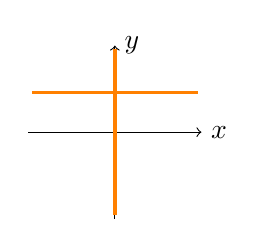
\begin{tikzpicture}[domain=-2:2,scale=.5]
		\draw[->] (-2.2,0) -- (2.2,0) node[right] {$x$};
		\draw[->] (0,-2.2) -- (0,2.2) node[right] {$y$};
		 \draw[color=orange,variable=\t,domain=-2.1:2.1,smooth,very thick]   plot ({\t},{1}) ;
		 \draw[color=orange,variable=\t,domain=-2.1:2.1,smooth,very thick]   plot ({0},{\t}) ;
	\end{tikzpicture} & & 
	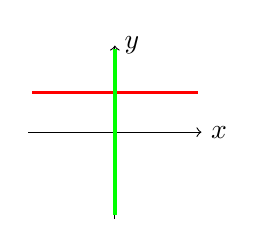
\begin{tikzpicture}[domain=-2:2,scale=.5]
		\draw[->] (-2.2,0) -- (2.2,0) node[right] {$x$};
		\draw[->] (0,-2.2) -- (0,2.2) node[right] {$y$};
		 \draw[color=red,variable=\t,domain=-2.1:2.1,smooth,very thick]   plot ({\t},{1}) ;
		 \draw[color=green,variable=\t,domain=-2.1:2.1,smooth,very thick]   plot ({0},{\t}) ;
	\end{tikzpicture}
\end{tabular}
	
	\end{center}
\end{frame}

\begin{frame}{Prime Decomposition: Example}
\begin{columns}[onlytextwidth]
	\begin{column}{0.6\textwidth}
	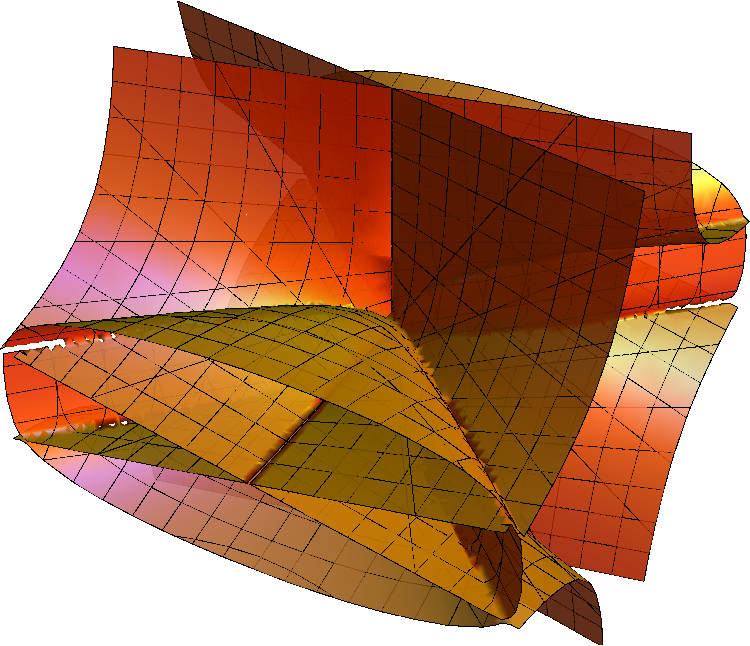
\includegraphics[width=0.8\textwidth]{complvar}
	\end{column}
	\begin{column}{0.4\textwidth}
	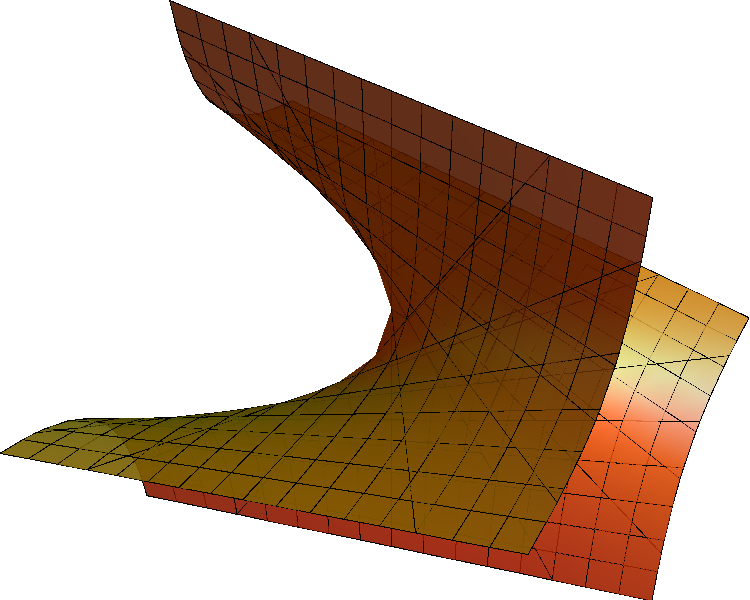
\includegraphics[width=0.8\textwidth]{complvar11}\\
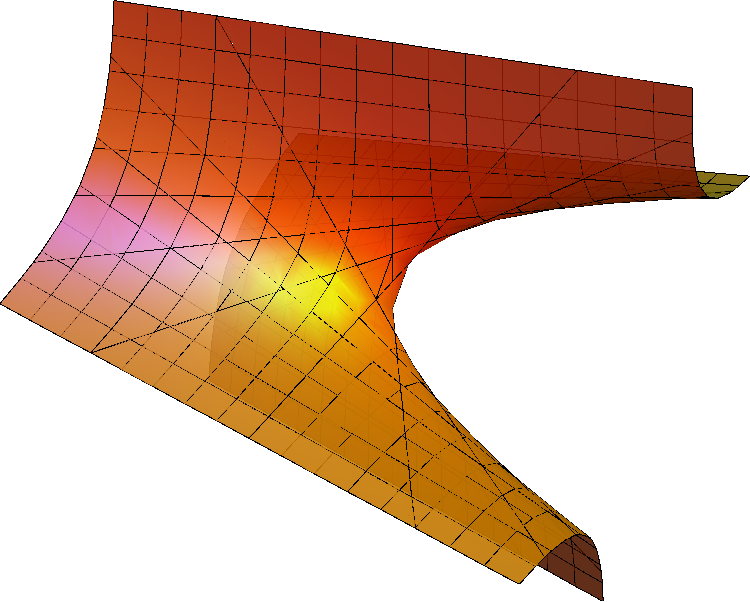
\includegraphics[width=0.8\textwidth]{complvar12}\\
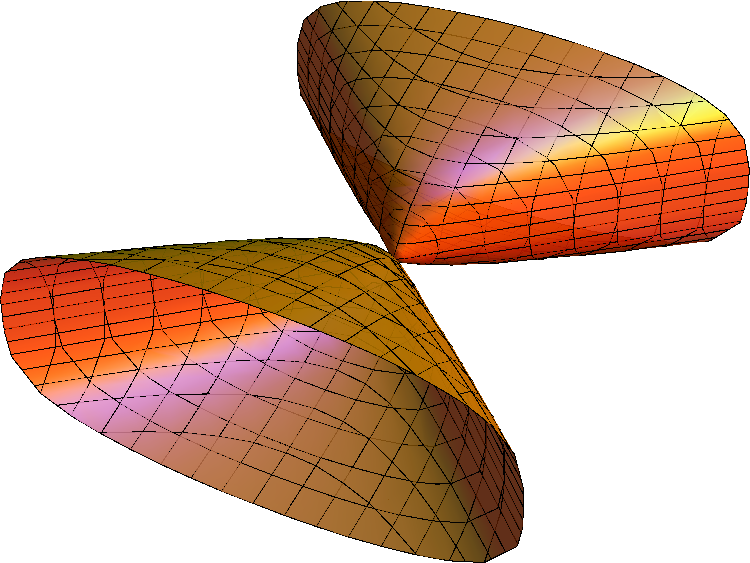
\includegraphics[width=0.8\textwidth]{complvar2}
	\end{column}
\end{columns}
\end{frame}

\begin{frame}{Prime Decomposition}
\begin{center}
\begin{tabular}{>{\Centering}p{0.35\textwidth} >{\Centering}p{0.1\textwidth} >{\Centering}p{0.35\textwidth} }
\toprule
\textbf{ALGEBRA} & & \textbf{GEOMETRY}\\
\midrule
prime ideal &$\leftrightarrow$ & irreducible variety\\
\bottomrule
\end{tabular}
\end{center}
\end{frame}



\subsection{Dimension}
\begin{frame}{Notions of Dimension}
Global concepts (same for irreducible varieties)\pause
\begin{itemize}[<+->]
\item Topological dimension (longest chain of embedded irreducible varieties)
\item Krull dimension (longest chain of prime ideals in the ring $\mathcal{O} (V) = \nicefrac{\kxn}{\I (V)}$)
\end{itemize}\pause
Local concepts
\begin{itemize}[<+->]
\item Tangent space:
\begin{align*}
T_p V = \ker \left( \frac{\partial F_i}{\partial x_j}\bigg|_p  \right)_{ij}
\end{align*}
\item Zariski tangent space ($\mathfrak{m}_p := \{ f \in \mathcal{O}(V) \; : \; f(p)=0\}$):
\begin{align*}
(T_p V)^* \cong \nicefrac{\mathfrak{m}_p}{\mathfrak{m}^2_p}
\end{align*}
\end{itemize}
\end{frame}

\begin{frame}{Singular Locus}
\begin{defn}[for irreducible varieties]
If local dimension in $p = $ global dimension, then $p $ is regular.\\
If local dimension in $p \neq$ global dimension, then $p$ is singular .
\end{defn}
\end{frame}

\begin{frame}{Singular Locus: Example}
\begin{columns}[onlytextwidth]
	\begin{column}{0.6\textwidth}
	\begin{itemize}[<+->]
	\item Defining equations: $\V (x) \cup \V (y,z) = \V (xy,xz)$
	\item Jacobian matrix
		\begin{align*}
		\frac{\partial F_i}{\partial x_j} = \begin{pmatrix}	y & x & 0 \\ z & 0 & x	\end{pmatrix}
		\end{align*}
	\end{itemize}
	\end{column}
	\begin{column}{0.4\textwidth}
	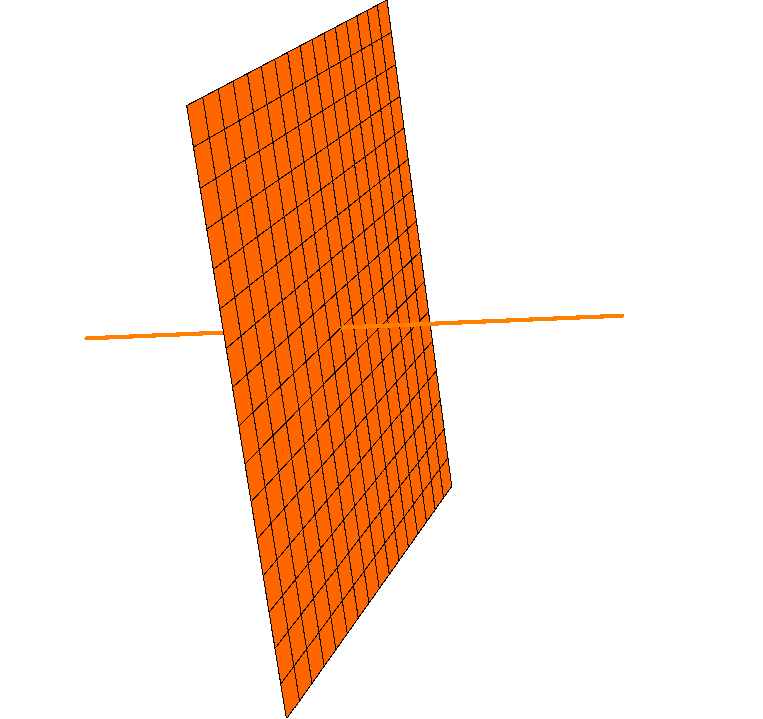
\includegraphics[width=\textwidth]{varietiesNotConstDim}
	\end{column}
\end{columns}
\pause
\begin{center}
\begin{tabular}{l | c | c}
		Locus & Rank & Dimension\\
		\toprule
		$x=y=z=0$  & $0$ & 3\\
		\midrule
		$x=0 \text{ and } (y\neq 0 \text{ or } z \neq 0)$ & $1$ & 2\\
		\midrule
		$x\neq 0, y=z=0$ & $2$ & 1\\
		\bottomrule
\end{tabular}
\end{center}

\end{frame}





\section{Application}

\subsection{Computations}
\begin{frame}{Given Equations}
\begin{align*}
0&=d_0 c_2^2 + b_0^2 c_1 - b_0 b_1 c_2\\
0&=d_1 b_0 c_2 - b_0^2 b_2-c_2^2 d_2
\end{align*}
\begin{align*}
0&=d_0 b_2 c_1 - b_0 b_2^2 - c_1^2 d_2\\
0&=d_1 c_1^2 - b_1 b_2 c_1 + b_2^2 c_2
\end{align*}
\begin{align*}
0&=d_0 c_1^3 c_2^2 + b_0^2 c_1^4-b_0 b_1 c_1^3 c_2 + c_2^3 (b_1 b_2 c_1 - b_2^2 c_2 - c_1^2 d_1)\\
0&=d_2 c_1^4 c_2^2+(b_0 c_1^2+c_2 (-b_1 c_1+b_2 c_2)) \times \\&\hspace{3em} \times (b_0 b_2 c_1^2+c_2 (-b_1 b_2 c_1+b_2^2 c_2+c_1^2 d_1))
\end{align*}
\end{frame}

\begin{frame}[fragile]
\frametitle{Extract Matter Curves}
\begin{lstlisting}
singular.lib('primdec.lib');
singular.lib('sing.lib');
R = singular.ring(0, '(b0,b1,b2,c1,c2,d0,d1,d2)', 'dp');
I1 = singular.ideal('d0*c2^2+b0^2*c1-b0*b1*c2','d1*b0*c2-b0^2*b2-c2^2*d2').std();
I2 = singular.ideal('d0*b2*c1-b0*b2^2-c1^2*d2','d1*c1^2-b1*b2*c1+b2^2*c2').std();
I3 = singular.ideal('d0*c1^3*c2^2-(-b0^2*c1^4+b0*b1*c1^3*c2+c2^3*(-b1*b2*c1+b2^2*c2+c1^2*d1))','d2*c1^4*c2^2+(b0*c1^2+c2*(-b1*c1+b2*c2))*(b0*b2*c1^2+c2*(-b1*b2*c1+b2^2*c2+c1^2*d1))').std();

# Extract the matter curves
I1pr = I1.minAssGTZ();
I2pr = I2.minAssGTZ();
I3pr = I3.minAssGTZ();
\end{lstlisting}
\end{frame}

\begin{frame}[fragile]
\frametitle{Matter Curves}
Every pair of the above equations defines two matter curves.
\begin{lstlisting}
# I1
CI1 = I1pr[2].std(); # c2 = 0 = b0
CI2 = I1pr[1].std(); # complicated

# I2
CI3 = I2pr[2].std(); # b2 = 0 = c1
CI4 = I2pr[1].std(); # complicated

# I3
CI5 = I3pr[2].std(); # c2 = 0 = c1
CI6 = I3pr[1].std(); # complicated
\end{lstlisting}
\end{frame}

\begin{frame}[fragile]
\frametitle{Allowed Yukawa Interactions}
\begin{columns}[onlytextwidth]
	\begin{column}{0.5\textwidth}
	\begin{itemize}
	\item $\ya$
	\item $\yb$
	\item  $\yc$
	\end{itemize}
	\end{column}
	\begin{column}{0.5\textwidth}
	\begin{itemize}
	\item $\yd$
	\item $\ye$
	\item $\yfs$.
	\end{itemize}
	\end{column}
\end{columns}
\pause
\vspace{1em}
\begin{lstlisting}
inters1 = (CI1+CI4+CI5).std();
inters2 = (CI2+CI3+CI5).std();
inters3 = (CI2+CI4+CI6).std();
inters4 = (CI1+CI2+CI6).std();
inters5 = (CI3+CI4+CI6).std();
singCI6 = singular.slocus(CI6).std();
inters6 = (CI5+singCI6).std();
inters61 = (CI5+CI6).std();
\end{lstlisting}
\end{frame}

\begin{frame}[fragile]
\frametitle{Compute Codimension}
\begin{lstlisting}
inters1pr = inters1.minAssGTZ();
inters2pr = inters2.minAssGTZ();
inters3pr = inters3.minAssGTZ();
inters4pr = inters4.minAssGTZ();
inters5pr = inters5.minAssGTZ();
inters6pr = inters6.minAssGTZ();
inters61pr = inters61.minAssGTZ();

inters1pr[1].std().dim()  # -> codim 3
inters2pr[1].std().dim()  # -> codim 3
inters3pr[1].std().dim()  # -> codim 3
inters3pr[2].std().dim()  # -> codim 4 # wrong codim
inters4pr[1].std().dim()  # -> codim 3
inters5pr[1].std().dim()  # -> codim 3
inters6pr[1].std().dim()  # -> codim 3
inters61pr[1].std().dim() # -> codim 3
inters61pr[2].std().dim() # -> codim 4 # wrong codim
\end{lstlisting}
\end{frame}


\subsection{Observe Fibre Enhancement}
\begin{frame}{Enhancement over Matter Curves}
\begin{itemize}[<+->]
\item Hypersurface equation:
\begin{gather*}
P_{T^2} = vw(c_1ws_1+c_2vs_0)+u(b_0v_2s^2_0+b_1vws_0s_1+b_2w_2s^2_1 )  \\
 + \: u_2(d_0vs^2_0s_1 +d_1ws_0s^2_1 +d_2us^2_0s^2_1)=0.
\end{gather*}
\item Consider e.g. $\mc{1}$: $c_2 = 0 = b_0$.
\item Then: 2-fold factorization
\begin{align*}
\left. P_{T^2} \right|_{\mc{1}} &\equiv \left. P_{T^2} \right|_{b_0 =0, c_2=0}  \\
%&=  s_1 (d_2 s_0^2 s_1 u^3 + d_0 s_0^2 u^2 v +  d_1 s_0 s_1 u^2 w + b_1 s_0 u v w + b_2 s_1 u w^2 + c_1 v w^2).
&=  s_1 (d_2 s_0^2 s_1 u^3 + d_0 s_0^2 u^2 v +  \ldots ).
\end{align*}
\item Meaning: Torus $\rightarrow$ two $\mathbb{P}^1$
\end{itemize}
\end{frame}


\begin{frame}{Enhancement over Intersection Loci}
\begin{itemize}[<+->]
\item Consider e.g. $\yd$: $c_2 = 0 = b_0$ and $d_1= \frac{ b_1 b_2 d_0 + b_1 c_1 d_2 \pm \sqrt{b_1^2 - 4 c_1 d_0} (b_2 d_0 - c_1 d_2)}{2 c_1 d_0}$.
\vspace{0.5em}
\item Then: 3-fold factorization
\begin{align*}
\left. P_{T^2} \right|_{\yd} = & \frac{1}{4 c_1 d_0} s_1 \left[ \left( b_1 \pm \sqrt{b_1^2 - 4 c_1 d_0} \right) s_0 u + 2 c_1 w \right]\\
		& \times \left[ \left(b_1 \mp \sqrt{b_1^2 - 4 c_1 d_0} \right) d_2 s_0 s_1 u^2+ \ldots\right]
\end{align*}
\item Meaning: Torus $\rightarrow$ three $\mathbb{P}^1$
\end{itemize}
\end{frame}


\begin{frame}{Enhancement over Intersection Loci}
\vspace{1em}
\begin{center}
\begin{tabular}{p{5cm} | c | c}
Locus & Physical content & $\dim_\C$\\
\toprule
Torus degenerates into one $\mathbb{P}^1$ & 7-branes & 2\\
\midrule
7-branes intersect / \newline degeneration into two $\mathbb{P}^1$s & matter curves & 1\\
\midrule
matter curves intersect / \newline degeneration into three $\mathbb{P}^1$s  & intersection locus & 0\\
\bottomrule
\end{tabular}
\end{center}
\hfill
\pause
\huge
\textcolor{green}{\ding{51}}
\end{frame}

\end{document}
